The simple application programming interface (API in abbreviated form) for 3D applications around which this thesis revolves offers a total of four particle based graphical effects. It is a small number of graphical effects but I designed the API in such a manner that it is very easy to extend, in other words other effects can be easily added to the API.\\

All the effects are enumerated bellow.

\begin{enumerate}
	\item Cone shaped particle system.
	
	\item Cylinder shaped particle system.
	
	\item Reversed cone shaped particle system.
	
	\item Fountain shaped particle system.
\end{enumerate}

The cone shaped particle system is a graphical effect in which all the particles are spawned exactly in the tip of the cone and each particle moves towards the base of the cone.\\

In the case of the cylinder shaped particle system all the particles are spawned at one end of an imaginary cylinder and move towards the other end of it.\\

The reversed cone shaped particle system is almost the same as the cone shaped particle system with the added difference that the particles are now spawned at the base of the cone and move towards the tip of the cone.\\

\newpage
The fountain particle system is somewhat based on the cone shaped particle system. The difference between the two of them is that in the case of the fountain particle system the particles are affected by gravity. In other words the fountain particle system sprays particles exactly like the cone shaped particle system does it only in the case of the fountain particle system the movement of the particle system is curved by a gravity force.\\

The following sections describe exactly how the four particle system types were implemented.\\

\newpage
\section{The Cone Shaped Particle System}
In order for the particle system to look like a cone (it will look roughly like a cone, it will actually have the resemblance of a sprayed flame) all the particles must be spawned exactly at the tip of an imaginary cone and must move towards random points which reside inside an imaginary sphere (the points can also lie on the sphere) which is placed exactly at the base of the cone.\\

\begin{figure}[h]
	\caption{Cone shaped particle system sketch}
	\centering
	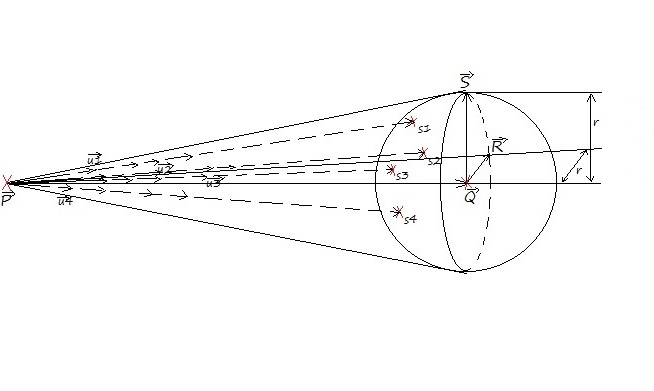
\includegraphics{cone.jpg}
\end{figure}

The sketch from Figure 3.1 shows how to conceive a cone shaped particle system. All the descriptions of the notations from the sketch are given bellow.\\

\begin{itemize}
	\item $\vec{P}$ represents the initial position vector, all the particles will have their position attribute initialized with this vector.
	
	\item $\vec{Q}$ represents the position vector of the center of the sphere. This vector is used to compute the destination position vectors which will lie inside or on the sphere.
	
	\item $\vec{s_1}, \vec{s_2}, \vec{s_3}$ and $\vec{s_4}$ represent the destination position vectors which lie inside or on the sphere.
	
	\item $\vec{u_1}, \vec{u_2}, \vec{u_3}$ and $\vec{u_4}$ represent series of direction vectors. These vectors are used to move each particle from the system in the particle update step. These vectors can be obtained by either normalizing the destination position vectors ($\vec{s_1}, \vec{s_2}$, ...) or by dividing them with a constant meant to scale them down.
	
	\item $r$ represents the size of the radius of the sphere. This radius is also the radius of the circle which forms the base of the cone. The value of this radius is used to compute the destination position vectors ($\vec{s_1}, \vec{s_2}$, ...).
\end{itemize}